\begin{figure}[!htb]
\centering
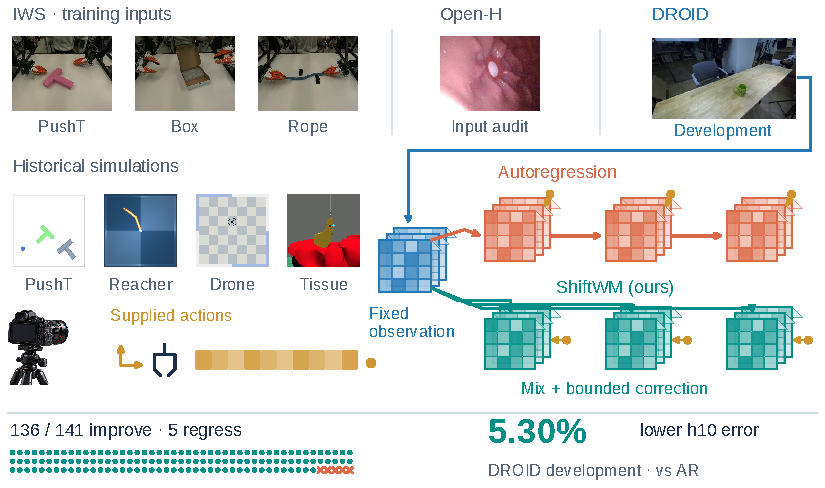
\includegraphics[width=\linewidth]{generated/editorial/teaser_benchmarks.pdf}
\caption[Forecast from a fixed observed reference.]{\textbf{Visual forecasting across the paper\textquotesingle s recorded and simulated settings.} Gallery: IWS PushT/Box/Rope are separate inputs to ongoing training; Open-H is a physical-phantom input audit only. Historical PushT, Reacher, drone and tissue simulations use distinct context models. Only DROID connects to the compared spatial decoder: autoregression reuses predictions; ShiftWM mixes a fixed observed reference with bounded corrections. Gold ports denote causal supplied-action prefixes; both routes share history. Three schematic steps depict ten forecast steps, not generated RGB; the camera is illustrative. Bottom: all 141 DROID development episodes. The 5.30\% reduction compares population mean native, training-standardized h10 feature MSE with matched autoregression. Uncertainty: Figure~\ref{fig:editorial-spatial}. Recorded images: DROID and Open-H (CC BY 4.0); IWS \citep{zhang2026rlawm}. Input-selection rules and simulator attribution accompany the editable figure.}
\label{fig:editorial-teaser}
\end{figure}
